\chapter{Derivazione funzione di costo DDPM}\label{appendix:details_loss}


\begin{figure}
    \centering
    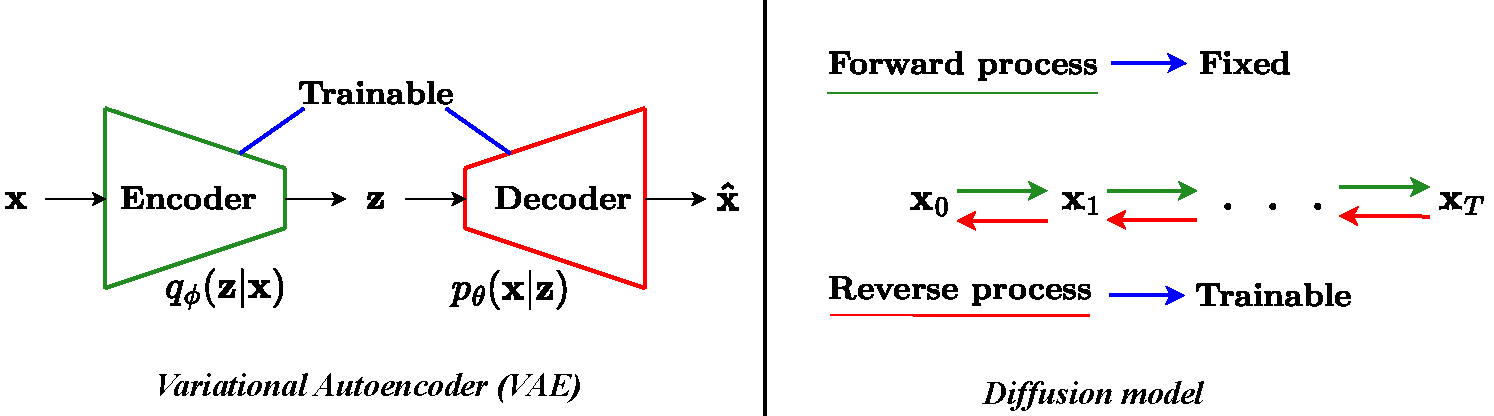
\includegraphics[keepaspectratio, scale=0.5]{VAE_vs_DIff.pdf}
    \caption{VAE e modello di diffusione a confronto. Fonte~\cite{nain2022}.}
    \label{fig:VAE_vs_Diff}
\end{figure}

Riguardando l'immagine $\mathbf{x}_0$ come un dato osservabile e $\mathbf{x}_1,\dots,\mathbf{x}_T$ come variabili \emph{latenti}, 
si ravvisa un'affinità con l'autoencoder variazionale (VAE) (Figura~\ref{fig:VAE_vs_Diff}).

\medskip

\noindent Similitudini:
\begin{itemize}
\item il processo di diffusione in avanti può essere riguardato come l'equivalente dell'encoder di un VAE, che converte 
i dati osservabili in variabili latenti.
\item il processo di diffusione inversa può essere riguardato come l'equivalente del decoder di un VAE, che, partendo dalle 
variabili latenti, fornisce in uscita i dati.
\end{itemize}

\noindent Differenze:
\begin{itemize}
    \item l'encoder e il decoder di un VAE sono due reti neurali che possono essere addestrate congiuntamente, 
    laddove il processo di diffusione in avanti in un DDPM è \emph{fisso} 
    (i.e non annovera parametri che possono essere appresi addestrando un'opportuna rete neurale).
    Soltanto il processo di diffusione inversa si avvale di una rete neurale.
\end{itemize}
Nel paper originale sui VAE (Kingma e Welling~\cite{kingmaVAE2022}), dette $\mathbf{x}$ una variabile osservabile e $\mathbf{z}$ una variabile latente, 
si perviene al seguente risultato:
\begin{equation}
\log p_{\bm{\theta}}(\mathbf{x})\geq \underbrace{\mathbb{E}_{q_{\bm{\phi}}(\mathbf{z}|\mathbf{x})}[\log p_{\bm{\theta}}(\mathbf{x}|\mathbf{z})]
-D_{KL}\bigl(q_{\bm{\phi}}(\mathbf{z}|\mathbf{x})\,\|\,p_{\bm{\theta}}(\mathbf{z})\bigr)}_{\text{Lower Bound Variazionale (ELBO)}} \label{eq:VAE_ELBO}
\end{equation}
Declinando la~\eqref{eq:VAE_ELBO} al contesto dei modelli di diffusione, con $\mathbf{x}_0$ e $\mathbf{x}_{1:T}$ che assurgono rispettivamente a 
dato osservabile e variabili latenti, si ha che~\cite{nain2022}:
\begin{align}
    \log p_{\bm{\theta}}(\mathbf{x})
    &\geq \mathbb{E}_{q(\mathbf{x}_{1:T}|\mathbf{x}_0)}[\log p_{\bm{\theta}}(\mathbf{x}_0|\mathbf{x}_{1:T})]\,-\,
    \mathcolor{blue}{D_{KL}\bigl(q(\mathbf{x}_{1:T}|\mathbf{x}_0)\,\|\,p_{\bm{\theta}}(\mathbf{x}_{1:T})\bigr)} \label{eq:elbo1}\\
    &= \mathbb{E}_{q(\mathbf{x}_{1:T}|\mathbf{x}_0)}[\log p_{\bm{\theta}}(\mathbf{x}_0|\mathbf{x}_{1:T})]\,-
    \,\mathcolor{blue}{\mathbb{E}_{q(\mathbf{x}_{1:T}|\mathbf{x}_0)}\biggl[\log\frac{q(\mathbf{x}_{1:T}|\mathbf{x}_0)}{p_{\bm{\theta}}(\mathbf{x}_{1:T})}\biggr]}\label{eq:elbo2}\\
    &= \mathbb{E}_q[\log p_{\bm{\theta}}(\mathbf{x}_0|\mathbf{x}_{1:T})]\,-\,\mathbb{E}_q\biggl[\log\frac{q(\mathbf{x}_{1:T}|\mathbf{x}_0)}{p_{\bm{\theta}}(\mathbf{x}_{1:T})}\biggr]\label{eq:elbo3}\\
    &=\mathbb{E}_q\biggl[\log p_{\bm{\theta}}(\mathbf{x}_0|\mathbf{x}_{1:T})\,-\,\log\frac{q(\mathbf{x}_{1:T}|\mathbf{x}_0)}{p_{\bm{\theta}}(\mathbf{x}_{1:T})}\biggr]\label{eq:elbo4}\\
    &= \mathbb{E}_q\biggl[\log p_{\bm{\theta}}(\mathbf{x}_0|\mathbf{x}_{1:T})\,+\,\log\frac{p_{\bm{\theta}}(\mathbf{x}_{1:T})}{q(\mathbf{x}_{1:T}|\mathbf{x}_0)}\biggr]\\
    &=\mathbb{E}_q\biggl[\log\frac{p_{\bm{\theta}}(\mathbf{x}_0|\mathbf{x}_{1:T})\,p_{\bm{\theta}}(\mathbf{x}_{1:T})}{q(\mathbf{x}_{1:T}|\mathbf{x}_0)}\biggr]\\
    &= \mathbb{E}_q\biggl[\log\frac{p_{\bm{\theta}}(\mathbf{x}_{0:T})}{q(\mathbf{x}_{1:T}|\mathbf{x}_0)}\biggr]
\end{align}
dove nel passaggio dalla~\eqref{eq:elbo1} alla~\eqref{eq:elbo2} si è sfruttata la definizione di \emph{divergenza di Kullback-Leibler}, 
dalla~\eqref{eq:elbo3} alla~\eqref{eq:elbo4} ci si è avvalsi della linearità dell'operatore di media statistica,
e infine delle proprietà dei logaritmi.

\medskip
\noindent Pertanto risulta che 
\begin{align}
    \log p_{\bm{\theta}}(\mathbf{x})&\geq\mathbb{E}_q\biggl[\log\frac{p_{\bm{\theta}}(\mathbf{x}_{0:T})}{q(\mathbf{x}_{1:T}|\mathbf{x}_0)}\biggr]\\
   \implies-\log p_{\bm{\theta}}(\mathbf{x})&\leq\mathbb{E}_q\biggl[-\log\frac{p_{\bm{\theta}}(\mathbf{x}_{0:T})}{q(\mathbf{x}_{1:T}|\mathbf{x}_0)}\biggr]\triangleq L_{vlb} 
\end{align}
Sostituendo le definizioni~\eqref{eq:forward_process} e~\eqref{eq:reverse_process} delle distribuzioni $q(\mathbf{x}_{1:T}|\mathbf{x}_0)$ e $p_{\bm{\theta}}(\mathbf{x}_{0:T})$ 
e usando le proprietà dei logaritmi:
\begin{equation}
    \begin{split}
    L_{vlb}&=\mathbb{E}_q\biggl[-\log p(\mathbf{x}_T)
    \mathcolor{Purple3}{-\log\frac{\prod_{t=1}^Tp_{\bm{\theta}}(\mathbf{x}_{t-1}|\mathbf{x}_t)}{\prod_{t=1}^Tq(\mathbf{x}_{t}|\mathbf{x}_{t-1})}}\biggr]\\
    &=\mathbb{E}_q\biggl[-\log p(\mathbf{x}_T)
    \mathcolor{Purple3}{-\log\prod_{t=1}^T\frac{p_{\bm{\theta}}(\mathbf{x}_{t-1}|\mathbf{x}_t)}{q(\mathbf{x}_{t}|\mathbf{x}_{t-1})}}\biggr]
    \end{split}
\end{equation}
Usando la poprietà dei logaritmi per cui il logaritmo di un prodotto è la somma dei logaritmi si ha:
\begin{equation}
    L_{vlb}=\mathbb{E}_q\biggl[-\log p(\mathbf{x}_T)
    \mathcolor{Purple3}{-\sum_{t=2}^T\log\frac{p_{\bm{\theta}}(\mathbf{x}_{t-1}|\mathbf{x}_t)}{q(\mathbf{x}_{t}|\mathbf{x}_{t-1})}
    -\log\frac{p_{\bm{\theta}}(\mathbf{x}_0|\mathbf{x}_1)}{q(\mathbf{x}_1|\mathbf{x}_0)}}\biggr] \label{eq:elbo5}
\end{equation}
Ricorrendo all'assunzione di Markov~\eqref{def:markov_property}, per cui l'ulteriore condizionamento a $\mathbf{x}_0$ è pleonastico, e alla legge di Bayes~\eqref{eq:Bayes}:
\begin{align}
    q(\mathbf{x}_t|\mathbf{x}_{t-1})&=q(\mathbf{x}_t|\mathbf{x}_{t-1},\mathbf{x}_0) \label{eq:markov_assumption}\\
    q(\mathbf{x}_t|\mathbf{x}_{t-1},\mathbf{x}_0)&=q(\mathbf{x}_{t-1}|\mathbf{x}_t,\mathbf{x}_0)\frac{q(\mathbf{x}_t|\mathbf{x}_0)}{q(\mathbf{x}_{t-1}|\mathbf{x}_0)}  \label{eq:bayesq}
\end{align}
\begin{oss}
Il condizionamento rispetto a $\mathbf{x}_0$ è essenziale: $q(\mathbf{x}_{t-1}|\mathbf{x}_t,\mathbf{x}_0)$ ammette un'espressione 
in forma chiusa, laddove $q(\mathbf{x}_{t-1}|\mathbf{x}_t)$ è intrattabile.
\end{oss}
\noindent Sostituendo il combinato disposto della~\eqref{eq:markov_assumption} e della~\eqref{eq:bayesq} nella~\eqref{eq:elbo5}:
\begin{equation}
    \mathbb{E}_q\biggl[-\log p(\mathbf{x}_T)
    \underbrace{-\sum_{t=2}^T\log\biggl(\frac{p_{\bm{\theta}}(\mathbf{x}_{t-1}|\mathbf{x}_t)}{q(\mathbf{x}_{t-1}|\mathbf{x}_t,\mathbf{x}_0)}\cdot 
    \frac{q(\mathbf{x}_{t-1}|\mathbf{x}_0)}{q(\mathbf{x}_t|\mathbf{x}_0)}\biggr)}
    -\log\frac{p_{\bm{\theta}}(\mathbf{x}_0|\mathbf{x}_1)}{q(\mathbf{x}_1|\mathbf{x}_0)}\biggr] \label{eq:intermediate_vlb} 
\end{equation}
Focalizzandosi sulla sommatoria centrale nella~\eqref{eq:intermediate_vlb} si ha che:
\begin{equation}
\begin{split}
    &-\sum_{t=2}^T\log\biggl(\frac{p_{\bm{\theta}}(\mathbf{x}_{t-1}|\mathbf{x}_t)}{q(\mathbf{x}_{t-1}|\mathbf{x}_t,\mathbf{x}_0)}\cdot 
    \frac{q(\mathbf{x}_{t-1}|\mathbf{x}_0)}{q(\mathbf{x}_t|\mathbf{x}_0)}\biggr)\\
    &= -\sum_{t=2}^T\log\frac{p_{\bm{\theta}}(\mathbf{x}_{t-1}|\mathbf{x}_t)}{q(\mathbf{x}_{t-1}|\mathbf{x}_t,\mathbf{x}_0)}
    \mathcolor{Blue3}{-\sum_{t=2}^T\log\frac{q(\mathbf{x}_{t-1}|\mathbf{x}_0)}{q(\mathbf{x}_t|\mathbf{x}_0)}} \label{eq:intermediate_steps}
\end{split}
\end{equation}
Isolando il secondo termine di sommatoria, risulta che:
\begin{equation}
    \begin{split}
    &\mathcolor{Blue3}{-\sum_{t=2}^T\log\frac{q(\mathbf{x}_{t-1}|\mathbf{x}_0)}{q(\mathbf{x}_t|\mathbf{x}_0)}}\\
    &=-\sum_{t=2}^T\log q(\mathbf{x}_{t-1}|\mathbf{x}_0)+\sum_{t=2}^T\log q(\mathbf{x}_t|\mathbf{x}_0) \\
    &=\mathcolor{Purple0}{-\sum_{t=1}^{T-1}\log q(\mathbf{x}_t|\mathbf{x}_0)}+\mathcolor{DeepSkyBlue1}{\sum_{t=2}^T\log q(\mathbf{x}_t|\mathbf{x}_0)}\\
    &=\mathcolor{Purple0}{-\log q(\mathbf{x}_1|\mathbf{x}_0)-\cancel{\sum_{t=2}^{T-1}\log q(\mathbf{x}_t|\mathbf{x}_0)}}+\mathcolor{DeepSkyBlue1}{\cancel{\sum_{t=2}^{T-1}\log q(\mathbf{x}_t|\mathbf{x}_0)}+\log q(\mathbf{x}_T|\mathbf{x}_0)} \\
    &=-\log q(\mathbf{x}_1|\mathbf{x}_0)+\log q(\mathbf{x}_T|\mathbf{x}_0) \label{eq:intermediate_steps2}
\end{split}
\end{equation}
Sostituendo il combinato disposto della~\eqref{eq:intermediate_steps} e della~\eqref{eq:intermediate_steps2} nella~\eqref{eq:intermediate_vlb} si ottiene che:
\begin{equation}
    \begin{split}
    L_{vlb}=\mathbb{E}_q\biggl[
        &\mathcolor{blue}{-\log p(\mathbf{x}_T)}-
           \sum_{t=2}^T\log\frac{p_{\bm{\theta}}(\mathbf{x}_{t-1}|\mathbf{x}_t)}{q(\mathbf{x}_{t-1}|\mathbf{x}_t,\mathbf{x}_0)}\\
        &\mathcolor{red}{-\log q(\mathbf{x}_1|\mathbf{x}_0)}\mathcolor{blue}{+\log q (\mathbf{x}_T|\mathbf{x}_0)}
        \mathcolor{red}{-\log\frac{p_{\bm{\theta}}(\mathbf{x}_0|\mathbf{x}_1)}{q(\mathbf{x}_1|\mathbf{x}_0)}}\biggr]
    \end{split}
\end{equation}
da cui, per le regole dei logaritmi:
\begin{equation}
    L_{vlb}=\mathbb{E}_q\biggl[\mathcolor{blue}{-\log \frac{p(\mathbf{x}_T)}{q(\mathbf{x}_T|\mathbf{x}_0)}}
    -\sum_{t=2}^T\log\frac{p_{\bm{\theta}}(\mathbf{x}_{t-1}|\mathbf{x}_t)}{q(\mathbf{x}_{t-1}|\mathbf{x}_t,\mathbf{x}_0)}
    \mathcolor{red}{-\log p_{\bm{\theta}}(\mathbf{x}_0|\mathbf{x}_1)}\biggr]
\end{equation}
Avvalendosi della definizione di \emph{divergenza di Kullback-Leibler}:
\begin{equation}
    \begin{split}
    D_{KL}\bigl(p_1(x)\,\|\,p_2(x)\bigr)
    &\triangleq\int_{-\infty}^{+\infty} p_1(x)\log\frac{p_1(x)}{p_2(x)}\,dx\\
    &=\mathbb{E}_{x\sim p_1(x)}\biggl[\log\frac{p_1(x)}{p_2(x)}\biggr] \\
    &=  \mathbb{E}_{p_1}\biggl[-\log\frac{p_2(x)}{p_1(x)}\biggr]  \label{eq:kullback-leibler}
    \end{split}
\end{equation}
si perviene, infine, al seguente risultato:
\begin{Mybox2}
\begin{equation}
    \begin{split}
    L_{vlb}= &\underbrace{-\log p_{\bm{\theta}}(\mathbf{x}_0|\mathbf{x}_1)}_{L_0}\\
    +&\sum_{t=2}^T \underbrace{D_{KL}\bigl(q(\mathbf{x}_{t-1}|\mathbf{x}_t,\mathbf{x}_0)\,\|\,p_{\bm{\theta}}(\mathbf{x}_{t-1}|\mathbf{x}_t)\bigr)}_{L_{t-1}}\\
    +&\underbrace{D_{KL}\bigl(q(\mathbf{x}_T|\mathbf{x}_0)\,\|\,p(\mathbf{x}_T)\bigr)}_{L_T}\label{eq:final_lvlb}
\end{split}
\end{equation}
\end{Mybox2}


\section*{Espressione analitica di $L_{t-1}$}\label{sec:detailed_loss_term}
Si dimostra che (Sohl-Dickstein et al.~\cite{sohl-dickstein2015}), sebbene $q(\mathbf{x}_{t-1}|\mathbf{x}_t)$ sia intrattabile, 
condizionando ulteriormente rispetto a $\mathbf{x}_0$ si perviene, 
(si veda~\cite{nain2022}), ad una distribuzione gaussiana, che, in quanto tale, è trattabile:
\begin{equation}
    q(\mathbf{x}_{t-1}|\mathbf{x}_t,\mathbf{x}_0) = \mathcal{N}(\mathbf{x}_{t-1}; \tilde{\bm{\mu}}_{t}(\mathbf{x}_t,\mathbf{x}_0),\tilde{\beta_t} \bm{I}) 
\end{equation}
dove 
\begin{align}
    \tilde{\bm{\mu}}_t(\mathbf{x}_t,\mathbf{x}_0) &=  \frac{\sqrt{\alpha_t}(1-\overline{\alpha}_{t-1})}{1-\overline{\alpha}_t}\mathbf{x}_t+
                                                      \frac{\sqrt{\overline{\alpha}_{t-1}}\beta_t}{1-\overline{\alpha}_t}\mathbf{x}_0 \label{eq:simplify}\\
    \tilde{\beta}_t &= \frac{1-\overline{\alpha}_{t-1}}{1-\overline{\alpha}_t}\beta_t
\end{align}
in cui $\alpha_t$ e $\overline{\alpha}_t$ sono definiti nella~\eqref{eq:alphas} e, dipendendo solo dagli iperparametri $\beta_t$, 
possono essere pre-calcolati.

Quindi $\tilde{\beta}_t$ e $\tilde{\bm{\mu}}_t(\mathbf{x}_t,\mathbf{x}_0)$ della distribuzione~\eqref{eq:true} sono i parametri 
che possono essere approssimati dalla media e varianza della distribuzione~\eqref{eq:approx}:
\begin{align}
    q(\mathbf{x}_{t-1}|\mathbf{x}_t,\mathbf{x}_0) &= \mathcal{N}(\mathbf{x}_{t-1}; \tilde{\bm{\mu}}_{t}(\mathbf{x}_t,\mathbf{x}_0),\tilde{\beta_t} \bm{I})\label{eq:true} \\
    p_{\bm{\theta}}(\mathbf{x}_{t-1}|\mathbf{x}_t)&=\mathcal{N}(\mathbf{x}_{t-1};\bm{\mu}_{\bm{\theta}}(\mathbf{x}_t,t),\bm{\Sigma}_{\bm{\theta}}(\mathbf{x}_t,t))\label{eq:approx}
\end{align}
addestrando un'opportuna rete neurale.

Pertanto, $L_{t-1}=D_{KL}\bigl(q(\mathbf{x}_{t-1}|\mathbf{x}_t,\mathbf{x}_0)\,\|\,p_{\bm{\theta}}(\mathbf{x}_{t-1}|\mathbf{x}_t)\bigr)$ 
risulta essere la divergenza di Kullback-Leibler tra due distribuzioni gaussiane e, in quanto tale, ammette un'espressione in forma chiusa.

\medskip
\noindent Sebbene nella~\eqref{eq:approx} la rete neurale possa apprendere sia la media che la varianza, Ho et al.~\cite{ho2020} hanno rilevato sperimentalmente
che l'apprendimento di quest'ultima degrada la qualità dei campioni prodotti dalla rete neurale a valle dell'addestramento.
Hanno deciso, quindi, di addestrare la rete neurale ad apprendere la sola media $\bm{\mu}_{\bm{\theta}}(\mathbf{x}_t,t)$, 
fissando la varianza $\bm{\Sigma}_{\bm{\theta}}(\mathbf{x}_t,t)=\beta_t\bm{I}$. 

Dunque, nella fase di addestramento la rete neurale deve apprendere la media $\bm{\mu}_{\bm{\theta}}(\mathbf{x}_t,t)$, cosicché 
la distribuzione~\eqref{eq:approx1} approssimi quanto più fedelmente possibile la~\eqref{eq:true1}:
\begin{align}
    q(\mathbf{x}_{t-1}|\mathbf{x}_t,\mathbf{x}_0) &= \mathcal{N}(\mathbf{x}_{t-1}; \tilde{\bm{\mu}}_{t}(\mathbf{x}_t,\mathbf{x}_0),\tilde{\beta_t} \bm{I})\label{eq:true1} \\
    p_{\bm{\theta}}(\mathbf{x}_{t-1}|\mathbf{x}_t)&=\mathcal{N}(\mathbf{x}_{t-1};\bm{\mu}_{\bm{\theta}}(\mathbf{x}_t,t),\beta_t\bm{I})\label{eq:approx1}
\end{align}

\noindent Inoltre, Ho et al.~\cite{ho2020} hanno osservato che, avvalendosi dell'artificio di riparametrizzazione~\eqref{eq:rep_trick} $\mathbf{x}_0$ può essere così riguardato:
\begin{equation}
  \mathbf{x}_0=\frac{1}{\sqrt{\overline{\alpha}}_t}(\mathbf{x}_t-\sqrt{1-\overline{\alpha}_t}\bm{\epsilon}) \label{eq:rep_trick3}
\end{equation}
dove $\bm{\epsilon}\sim\mathcal{N}(\bm{0},\bm{I})$.
Dal combinato disposto della~\eqref{eq:simplify} e della~\eqref{eq:rep_trick3} risulta che 
$\tilde{\bm{\mu}}_t$ dipende solo da $\mathbf{x}_t$:
\begin{equation}
    \tilde{\bm{\mu}}_t(\mathbf{x}_t)=\frac{1}{\sqrt{\alpha_t}}\biggl(\mathbf{x}_t-\frac{1-\alpha_t}{\sqrt{1-\overline{\alpha}_t}}\bm{\epsilon}\biggr) \label{eq:true_mean}
\end{equation}
Quindi in ogni passo della diffusione inversa la rete neurale deve approssimare la media nella~\eqref{eq:true_mean}. 
Tuttavia, poiché $\mathbf{x}_t$ è disponibile come input del generico passo di diffusione inversa e gli $\alpha_t$ sono noti a monte della fase di training,
allora apprendere la suddetta media si traduce nell'apprendere il rumore $\bm{\epsilon}_t$ additivo che è stato aggiunto nel corrispondente passo di diffusione in avanti:
\begin{equation}
    \bm{\mu}_{\bm{\theta}}(\mathbf{x}_t,t)=\frac{1}{\sqrt{\alpha_t}}\biggl(\mathbf{x}_t-\frac{1-\alpha_t}{\sqrt{1-\overline{\alpha}_t}}\bm{\epsilon}_{\bm{\theta}}(\mathbf{x}_t,t)\biggr) \label{eq:learned_mean}
\end{equation}

\noindent Quindi il termine $L_{t-1}$ risulta essere:
\begin{equation}
L_{t-1}=D_{KL}\biggl(\mathcal{N}\Bigl(\mathbf{x}_{t-1}; \tilde{\bm{\mu}}_{t}(\mathbf{x}_t,\mathbf{x}_0),\tilde{\beta_t} \bm{I}\Bigr)\,\big\|\,\mathcal{N}\Bigl(\mathbf{x}_{t-1};\bm{\mu}_{\bm{\theta}}(\mathbf{x}_t,t),\beta_t\bm{I}\Bigr)\biggr)
\label{eq:kl_div_gaussians}
\end{equation}
dove $\bm{\mu}_{\bm{\theta}}(\mathbf{x}_t,t)$ è quella della~\eqref{eq:learned_mean}.

Ma la~\eqref{eq:kl_div_gaussians} è la divergenza di Kullback-Leibler tra due distribuzioni gaussiane e, a valle di alcuni calcoli (si veda~\cite{nain2022}), 
si perviene alla seguente riformulazione per $L_{t-1}$:
\begin{equation}
L_{t-1}=\mathbb{E}_{\mathbf{x}_0,\bm{\epsilon}}\biggl[\underbrace{\frac{(1-\alpha_t)^2}{2\alpha_t\beta_t(1-\overline{\alpha}_t)}}_{\text{termine di scalatura}}\Big\Vert \bm{\epsilon}-
\bm{\epsilon}_{\bm{\theta}}(\underbrace{\sqrt{\overline{\alpha}_t}\mathbf{x}_0+\sqrt{1-\overline{\alpha}_t}\bm{\epsilon}}_{\mathbf{x}_t},t)\Big\Vert^2\biggr] \label{eq:almost_final}
\end{equation}

\noindent Infine Ho et al.~\cite{ho2020} hanno osservato sperimentalmente che, ignorando il termine di scalatura nella~\eqref{eq:almost_final}, 
si ottengono prestazioni migliori a valle dell'addestramento del modello. 

Pertanto, ognuno degli $L_{t-1}$ nella~\eqref{eq:final_lvlb} esibisce la seguente espressione semplificata:
\begin{Mybox2}
\begin{equation}
    L_{t-1}^{\text{simple}}=\Vert \bm{\epsilon}-
    \bm{\epsilon}_{\bm{\theta}}(\underbrace{\sqrt{\overline{\alpha}_t}\mathbf{x}_0+\sqrt{1-\overline{\alpha}_t}\bm{\epsilon}}_{\mathbf{x}_t},t)\Vert^2 +C
\end{equation}
\end{Mybox2}

\smallskip
\noindent dove $C$ è una costante che non dipende da $\bm{\theta}$ e, quindi, può essere ignorata durante l'addestramento.